% This is LLNCS.DEM the demonstration file of
% the LaTeX macro package from Springer-Verlag
% for Lecture Notes in Computer Science,
% version 2.4 for LaTeX2e as of 16. April 2010
%
\documentclass{llncs}

\usepackage{amsmath}
\usepackage{amsfonts}
\usepackage{latexsym}
\usepackage{graphicx}
\usepackage{hyperref}
\usepackage{wrapfig}
\usepackage{scalefnt}
\usepackage{tikz}
\usepackage{url}
\usepackage{makeidx}  % allows for indexgeneration
%
\newcommand{\icon}[1]{\tikz[baseline=-3pt] \node[inner sep=0pt,outer sep=0pt]{\includegraphics[height=1.1em]{images/#1}};}

\begin{document}
%
\frontmatter          % for the preliminaries
%
\pagestyle{headings}  % switches on printing of running heads
%
\mainmatter              % start of the contributions
%
\title{Scientific workflow management with the ADAMS system.}
%
\titlerunning{ADAMS: scientific workflow}  % abbreviated title (for running head)
%                                     also used for the TOC unless
%                                     \toctitle is used
%
\author{Joaquin Vanschoren\inst{1} \and Peter Reutemann\inst{2}}
%
\authorrunning{Joaquin Vanschoren et al.} % abbreviated author list (for running head)
%
%%%% list of authors for the TOC (use if author list has to be modified)
\tocauthor{Joaquin Vanschoren and Peter Reutemann}
%
\institute{Leiden University, Leiden, NL,\\
\email{joaquin@liacs.nl}
\and
University of Waikato, Hamilton, NZ \\
\email{fracpete@waikato.ac.nz}}

\maketitle              % typeset the title of the contribution

\begin{abstract}
We demonstrate the practical use of a novel, flexible workflow engine, the Advanced Data mining And Machine learning System (ADAMS), aimed at quickly building and maintaining real-world, complex knowledge workflows. While most workflow engines allow users to manually arrange and connect different operators on a canvas, it becomes quite tedious to do so in complex, real-world settings with tens, maybe hundreds of operators. ADAMS automatically arranges workflows in a very compact way and offers a range of \emph{control operators} (e.g. branches and while-loops) to direct the data flow. It contains an extensive library of operators, and a plug-in architecture to easily add new ones.
\keywords{scientific workflows, workflow engines, machine learning, data mining}
\end{abstract}
%
\section{Introduction}
Many of today's data mining platforms offer \emph{workflow engines} allowing the user to design and run knowledge workflows, from cleaning raw data to building models and making predictions. Most of these systems, such as Kepler \cite{kepler}, RapidMiner \cite{rm} and KNIME \cite{knime2007}, are data-driven, i.e. data is passed from one operator to the next, and represent these dependencies in a directed graph.\footnote{For an in-depth overview and comparison of scientific workflow systems, see \cite{deelman,bowers}}. Many of them take a ``canvas''-based approach, in which the user places the various operators on a large canvas and then connects the various inputs and outputs manually, thus introducing each dependency as a line on the canvas. 

Though this is a very intuitive approach to design, it is also a very time consuming one. When inserting additional pre-processing steps, potentially in multiple places in numerous processing branches, the user ends up moving and rearranging a lot of actors in order to keep the design tidy, and needs to double-check if no crucial connections are broken. Moreover, many scientific data analyses are complex and can involve hundreds of independent steps and large amounts of heterogeneous data\cite{bowers}. On a canvas, this leads to very complex graphs and oversight is easily lost, even with useful features such as zooming, hierarchical workflows or operators with internal workflows.

In this paper, we present the ADAMS framework (Advanced Data mining And Machine learning System), specifically aimed at quickly building and maintaining real-world, complex knowledge workflows. It entirely takes away the need to layout operators and connect inputs to outputs, and instead represents workflows in a very compact, automatically layouted tree structure in which operators can quickly be dropped in or pulled out, thus allowing quick workflow prototyping. In the remainder of this paper, we will first discuss how ADAMS supports complex scientific workflows in compact trees in Section \ref{representation}. Next, we will show how easy it is to write new operators in Section \ref{newactors}. Finally, Section \ref{examples} provides a brief overview of supported tasks and some real-world examples. 

%that uses much more compact and simplified workflow representation to allow the user to focus on quick prototyping

\section{Workflow representation}
\label{representation}

\begin{wrapfigure}{rt}{5cm}
  \centering
  \vspace{-40pt}
  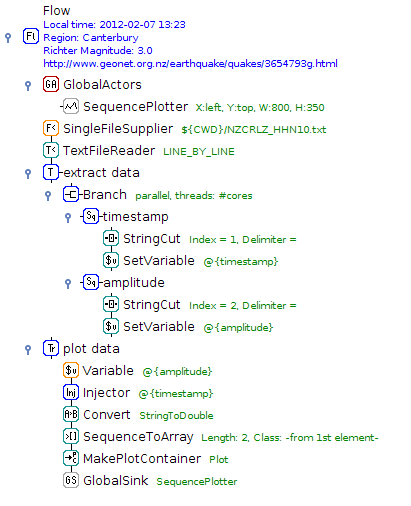
\includegraphics[width=5cm]{images/geonet_flow.png}
  \vspace{-20pt}
  \caption{Flow for processing and visualizing seismic data.}
  \label{flow}
  \vspace{-20pt}
\end{wrapfigure}

Figure \ref{flow} shows an example of an ADAMS workflow. It reads a file with earthquake data and plots it.\footnote{With the right actor, this can of course be done in much fewer steps, but we want to illustrate ADAMS control actors here.} As in canvas-based systems, operators (called `actors' in ADAMS) are dragged from a library into the workflow. However, in ADAMS, they will automatically `snap' into the tree structure. Actors are represented by a small node with a (custom) name and a list of parameter settings (options). They are
color-coded based on whether they are a \emph{source} (only output, e.g. \texttt{SingleFileSupplier}~\icon{source}), \emph{sink} (only input, e.g. \texttt{SequencePlotter}~\icon{sink}), \emph{transformer} (input and output, e.g. \texttt{Convert}~\icon{transformer}) or \emph{standalone} (neither input nor output, e.g. \texttt{GlobalActors}~\icon{standalone}). Each branch can be collapsed, and each actor can be clicked to open a settings dialog.

\paragraph{Tokens.} Data are passed as \emph{tokens} wrapping a single Java object (e.g. a string or an entire dataset), as well as provenance information, i.e. the trace of actors preceding the data. Transformer actors can receive a single token (e.g. a file name) and emit many (e.g. one for each read line), or vice versa, collect tokens and emit a single array (e.g., the \texttt{SequenceToArray} actor). Actors that produce different kinds of output can attach a key to a token (creating a key-value pair), and many such pairs can be combined in a \emph{container}. For instance, \texttt{MakePlotContainer} builds a container where data is labeled 'X' or 'Y' so it can be plotted. A \texttt{ContainerValuePicker} actor can later extract the token with a given key.

\paragraph{Control actors} control how data is passed between actors, and thus replace hand-drawn connections. A \texttt{Sequence} \icon{sequence} executes all its sub-actors in sequence, passing the input to the first sub-actor in line. A \texttt{Branch}~\icon{branch} channels its input to all underlying actors and executes them in parallel. A \texttt{Tee}~\icon{tee} splits off its input to its sub-flow and executes it before passing it on, a \texttt{Trigger}~\icon{trigger} starts its sub-flow upon receiving an input (but does not forward the data to its sub-flow), and an \texttt{Injector}~\icon{injector} injects a certain value into the flow, in addition to passing on its input. Some control actors have conditions, such as the \texttt{Conditional Tee}, only executes its sub-flow if a stated condition holds, or the \texttt{If-Then-Else} actor, which executes one of two sub-workflows depending on a boolean test. ADAMS defines over 20 such control actors.

\paragraph{N-to-M semantics.} The drawback of a tree representation is that it cannot represent N-to-M relationships. ADAMS offers three ways of dealing with this shortcoming. First, any token can be written to a \emph{variable}. In Figure \ref{flow}, the \texttt{SetVariable} actor assigns its input value to a certain variable, e.g. \emph@\{timestamp\}, which can then be used at any point in the workflow. It can be (re)introduced in the flow by the \texttt{Variable} source actor, or be part of another actor's option settings, thus dynamically changing the behavior of the flow. Similarly, any token (also complex objects) can be stored as a key-value pair by the \texttt{SetStorageValue} actor and afterwards be reintroduced by the \texttt{StorageValue} source actor. Finally, actors and entire sub-flows can be defined as \emph{global} by dragging them under \texttt{GlobalActors}, and called simply by inserting a \texttt{GlobalSink}/\texttt{Source}/\texttt{Transformer} actor referencing their name, such as \texttt{SequencePlotter} in Fig. \ref{flow}.

\paragraph{Interactivity} Actors can interact with the user. For instance, they can ask the user to locate an undefined file, or even display a number of results, and allow the user to make a subselection before proceeding.

\section{Finding and building new actors}
\label{newactors}
ADAMS contains an extensive library of operators. Table \ref{table} provides a short overview of known tools which are currently fully supported in ADAMS.

\begin{table}[htdp]
\caption{default}
\begin{center}
\begin{tabular}{|l|l|}
\hline
Task & Support for \\
\hline
Machine learning & WEKA, MOA, parameter optimization, experiment generation \\
Data Streams & MOA, Twitter \\
Spreadsheets & MS Excel, ODF, CSV \\
Graphics & BMP, JPG, PNG, TIF, PDF \\
Imaging & ImageJ, JAI, ImageMagick, Gnuplot \\
Scripting & Groovy, Jython \\
Documentation & DocBook, HTML \\
Other & HTTP, FTP, SFTP, SSH, Email, tar/zip/bzip2/gzip/lzma, Java code generation \\
\hline
\end{tabular}
\end{center}
\label{table}
\end{table}%

In addition, ADAMS sports a plug-in architecture to easily write and add new actors on the fly. A new actor can be written as a single Java class implementing a simple interface for receiving and emitting tokens and defining and setting options. Next, it has to be dropped in a specific folder (together with an optional icon) where it will be found and made directly available.

\section{Examples}
\label{examples}

For more examples and videos, please refer to the following URL: \\
\url{http://www.cs.waikato.ac.nz/~fracpete/adams-demo/}

%
% ---- Bibliography ----
%
\begin{thebibliography}{5}
\bibitem{kepler}
Lud\"{a}scher, B., I. Altintas, C. Berkley, D. Higgins, E. Jaeger, M. Jones, E. A. Lee, J. Tao, and Y. Zhao:
Scientific workflow management and the Kepler system.
Concurrency and Computation: Practice and Experience, 18:1039�1065 (2006).

\bibitem{rm}
Mierswa, I., M. Wurst, R. Klinkenberg, M. Scholz, and T. Euler. Yale: 
Rapid prototyping for complex data mining tasks. 
In Proceedings of the 12th ACM SIGKDD International Conference on Knowledge Discovery and Data Mining (2006).

\bibitem{knime2007}
Berthold M. R., Cebron, N., Dill, F., Gabriel, T. R., K\"{o}tter, T., Meinl, T., Ohl P., Sieb, C., Thiel, K., Wiswedel, B.:
KNIME: The Konstanz Information Miner. In \emph{Data Analysis, Machine Learning and Applications}, pp. 319-326 (2008). 

\bibitem{deelman}
Deelman, E., Gannon, D., Shields, M., Taylor, I.: Workflows and e-Science: An overview of workflow system features and capabilities. Future Generation Computer Systems 25(2009): 528-540.

\bibitem{bowers}
Bowers, S.: Scientific Workflow, Provenance, and Data Modeling Challenges and Approaches. Data Semantics (2012) 1:19-30.

%\bibitem{holmes2010}
%Holmes, G., Fletcher, D., Reutemann, P.: Predicting Polycyclic Aromatic Hydrocarbon Concentrations in Soil and Water Samples. Proceedings of the International Congress on Environmental Modelling and Software (IEMSS), Ottawa, Canada (2010).

\end{thebibliography}

\end{document}
